\subsection{Treatment of Statistical Uncertainties on Background Rate
  Predictions}%
\label{sec:barlow_beeston}

The predicted background rate in a given bin $b$ of a channel $c$ is
determined from a finite sample of events, e.g.\ from MC simulation,
and thus does not directly correspond to the true expected rate. The
background rate estimates are subject to uncertainties that have to be
considered when performing inference, particularly when bins are only
sparsely populated with events.

This uncertainty is included in the likelihood function, employing the
method proposed by Barlow and Beeston~\cite{barlow1993}, by replacing
the expected background rate from the prediction using the finite
sample with the true expected rate that has to be simultaneously
inferred. In practice this is done by performing the substitution
$\nu_{cb} \rightarrow \gamma_{cb} \nu_{cb}$ that introduces new
nuisance parameters $\gamma_{cb}$ specifying the relative difference
between the predicted and true expected rates. Initially it was
proposed to introduce one such nuisance parameter for every background
source~\cite{barlow1993}, however, a simplified version proposed in
Ref.~\cite{conway2011} is used such that only the combined uncertainty
on the total background prediction is considered instead.

The $\gamma$ nuisance parameters are constrained by auxiliary
measurements using the observed samples of events entering the
bins. These measurements contribute terms of the form
\begin{align*}
  \pois(m_{cb} | \gamma_{cb} \tau_{cb})
  \qquad \text{with} \qquad
  \tau_{cb} = \frac{( \sum_i w_i )^2}{\sum_i w_i^2} = \text{const.}
\end{align*}
to the likelihood function~\cite{cranmer2012}, where the sums go over
all events contributing to bin $b$ in channel $c$ with event weights
$w_i$. This corresponds to a measurement of the effective number of
events based on the observed value $m_{cb}$, which is nominally equal
to $\tau_{cb}$,\footnote{It should be noted that $m_{cb}$ are generally
  not integer-valued quantities and thus do not agree with the support
  of the Poisson distribution. Thus the factorial term in the Poisson
  PMF is replaced by the continuous gamma function to generalise the
  distribution to $\mathbb{R}^+$.} from the finite sample.

This approach is based on the approximation of the \emph{compound
  Poisson distribution} (CPD) that describes the distribution of the
sum of a Poisson number of random weights with a \emph{scaled Poisson
  distribution} (SPD)~\cite{Bohm:2013gla}. The CPD describes the
distribution of rate predictions based on a finite sample of weighted
events and can be defined as
\begin{align*}
  X = \sum_{i = 1}^{N} W_i \quad \text{with} \quad N \sim \pois(\lambda) \quad \text{and} \quad \text{i.i.d.\ } W_i \text{ (independent of }N\text{)} \,\text{.}
\end{align*}
It can be approximated, see for example Ref.~\cite{Bohm:2013gla},
using a scaled Poisson distribution defined by
\begin{align*}
  \tilde{X} = s \cdot \tilde{N} \quad \text{with} \quad \tilde{N} \sim \pois(\tilde{\lambda})
\end{align*}
with
\begin{align*}
  s = \frac{\expect(W^2)}{\expect(W)} \qquad \tilde{\lambda} = \frac{\lambda \expect(W)^2}{\expect(W^2)}
\end{align*}
where $\expect(W)$ and $\expect(W^2)$ are the first and second moment
of the weight distribution. The Barlow--Beeston method makes the
assumption that the expectation values can be approximated by sample
averages such that
\begin{align*}
  s = \frac{\sum_i w_i^2}{\sum_i w_i} \qquad \tilde{\lambda} = \frac{\lambda}{n} \frac{(\sum_i w_i)^2}{\sum_i w_i^2}
\end{align*}
with sample size $n$. Comparing the equation for $\tilde{\lambda}$
with the constraint term entering the likelihood function illustrates
the connection to a measurement of the effective number of events. A
number of $\tilde{N}$ events contribute with equal weights given by
$s$ to the sum, thus $\tilde{N}$ can be referred to as an effective
number of events.

These relationships will be needed in the context of the statistical
interpretation of the results in~\Cref{sec:toys_global_observables}.

%%% Local Variables:
%%% mode: latex
%%% TeX-master: "../../phd_thesis"
%%% End:


% ------------------------------------------------------------------------------
\clearpage
\subsection{Tables of Upper Limits}%
\label{app:limit_tables}
% ------------------------------------------------------------------------------

\begin{table}[htbp]
  \centering

  % Workspaces: comb_2022_01_29
  \setlength{\tabcolsep}{1.2em}

\begin{tabular}{
  S[round-mode=places, round-precision=1, table-format=4.0]
  S[round-mode=figures, round-precision=2, table-format=4.0]
  S[round-mode=figures, round-precision=2, table-format=4.1]
  S[round-mode=figures, round-precision=2, table-format=4.1]
  S[round-mode=figures, round-precision=2, table-format=4.1]
  S[round-mode=figures, round-precision=2, table-format=4.1]
  S[round-mode=figures, round-precision=2, table-format=4.1]
  }
  \toprule
  & \multicolumn{6}{c}{Upper limit on $\sigma(\pp \to X \to \HH)$ at \SI{95}{\percent}~CL / \si{\femto\barn}} \\ \cmidrule{2-7}
  {$\mX / \si{\GeV}$} & {Observed} & {-2$\sigma$} & {-1$\sigma$} & {Expected} & {+1$\sigma$} & {+2$\sigma$} \\
  \midrule
  251 & 638.439474 &   181.597753 &   243.795325 & 338.343637 &   470.876453 &   631.243225 \\
  260 & 896.941144 &   388.414694 &   521.447460 & 723.674376 &  1007.145358 &  1350.149661 \\
  280 & 486.649582 &   451.329066 &   605.910122 & 840.893212 &  1170.280064 &  1568.843286 \\
  300 & 536.855730 &   354.268351 &   475.605929 & 660.054657 &   918.605115 &  1231.455197 \\
  325 & 335.203789 &   253.311729 &   340.071473 & 471.957446 &   656.828218 &   880.524732 \\
  350 & 225.955597 &   188.434655 &   252.973879 & 351.081802 &   488.604294 &   655.008651 \\
  375 & 128.478432 &   116.329338 &   156.172355 & 216.738867 &   301.637796 &   404.366822 \\
  400 &  79.740112 &    76.742967 &   103.027578 & 142.983568 &   198.991758 &   266.762541 \\
  450 &  47.487654 &    36.311632 &    48.748434 &  67.653973 &    94.154757 &   126.221118 \\
  500 &  46.443591 &    22.921119 &    30.771645 &  42.705456 &    59.433639 &    79.675001 \\
  550 &  25.460027 &    17.653045 &    23.699246 &  32.890250 &    45.773712 &    61.362902 \\
  600 &  21.061634 &    14.051405 &    18.864037 &  26.179858 &    36.434787 &    48.843412 \\
  700 &  25.438956 &    10.020276 &    13.452240 &  18.669266 &    25.982217 &    34.831001 \\
  800 &  30.810426 &     8.174691 &    10.974539 &  15.230667 &    21.196681 &    28.415652 \\
  900 &  30.585851 &     7.193141 &     9.656806 &  13.401892 &    18.651557 &    25.003732 \\
  1000 &  30.462079 &     6.544590 &     8.786125 &  12.193545 &    16.969887 &    22.749335 \\
  1100 &  27.986994 &     7.199577 &     9.665446 &  13.413883 &    18.668245 &    25.026104 \\
  1200 &  24.592590 &     7.380353 &     9.908137 &  13.750695 &    19.136990 &    25.654490 \\
  1400 &  27.352079 &    10.649380 &    14.296812 &  19.841379 &    27.613459 &    37.017797 \\
  1600 &  33.882981 &    16.663186 &    22.370359 &  31.045995 &    43.207043 &    57.922100 \\
  \bottomrule
\end{tabular}

%%% Local Variables:
%%% mode: latex
%%% TeX-master: "../phd_thesis"
%%% End:

  \caption{$\text{CL}_\text{s}$ upper limits on the cross section of
    $\PX \ra \PHiggs \PHiggs \ra \bbtautau$ from the combined fit of
    all channels. Limits are in fb.}%
  \label{tab:comb_limits_resonant}
\end{table}

\begin{table}[htbp]
  \centering

  % Workspaces: comb_2022_01_29
  \setlength{\tabcolsep}{1.2em}

\begin{tabular}{
  S[round-mode=places, round-precision=1, table-format=4.0]
  S[round-mode=figures, round-precision=2, table-format=4.0]
  S[round-mode=figures, round-precision=2, table-format=4.1]
  S[round-mode=figures, round-precision=2, table-format=4.1]
  S[round-mode=figures, round-precision=2, table-format=4.1]
  S[round-mode=figures, round-precision=2, table-format=4.1]
  S[round-mode=figures, round-precision=2, table-format=4.1]
  }
  \toprule
  & \multicolumn{6}{c}{Upper limit on $\sigma(\pp \to X \to \HH)$ at \SI{95}{\percent}~CL / \si{\femto\barn}} \\ \cmidrule{2-7}
  {$\mX / \si{\GeV}$} &  {Observed} & {-2$\sigma$} & {-1$\sigma$} &  {Expected} & {+1$\sigma$} & {+2$\sigma$} \\
  \midrule
  251 &  973.495799 &   265.045066 &   355.823501 &  493.818400 &   687.252341 &   921.310423 \\
  260 & 1627.925794 &   557.380325 &   748.284137 & 1038.482489 &  1445.267171 &  1937.482972 \\
  280 &  885.081013 &   554.703191 &   744.690080 & 1033.494591 &  1438.325460 &  1928.177118 \\
  300 &  900.688379 &   426.880001 &   573.087206 &  795.340965 &  1106.884516 &  1483.857065 \\
  325 &  427.179604 &   285.774280 &   383.652509 &  532.440009 &   741.002448 &   993.366246 \\
  350 &  262.632595 &   216.567956 &   290.742890 &  403.498330 &   561.552936 &   752.801470 \\
  375 &  153.878061 &   126.844843 &   170.289441 &  236.330819 &   328.904125 &   440.919267 \\
  400 &  102.277962 &    84.818611 &   113.869145 &  158.029694 &   219.931613 &   294.833899 \\
  450 &   62.479143 &    41.225854 &    55.345787 &   76.809901 &   106.897159 &   143.303211 \\
  500 &   55.685134 &    28.092274 &    37.713931 &   52.340087 &    72.842259 &    97.650205 \\
  550 &   25.524188 &    21.202297 &    28.464123 &   39.503034 &    54.976794 &    73.700285 \\
  600 &   26.608906 &    17.384295 &    23.338449 &   32.389529 &    45.076853 &    60.428713 \\
  700 &   32.164818 &    12.811085 &    17.198906 &   23.868959 &    33.218685 &    44.531999 \\
  800 &   33.258635 &    10.820855 &    14.527018 &   20.160863 &    28.058088 &    37.613854 \\
  900 &   42.358711 &     9.759847 &    13.102613 &   18.184048 &    25.306933 &    33.925736 \\
  1000 &   43.661054 &     9.557592 &    12.831085 &   17.807216 &    24.782492 &    33.222686 \\
  1100 &   35.580690 &    10.783233 &    14.476511 &   20.090768 &    27.960536 &    37.483079 \\
  1200 &   35.027829 &    11.710499 &    15.721367 &   21.818402 &    30.364903 &    40.706303 \\
  1400 &   34.671442 &    16.796855 &    22.549810 &   31.295041 &    43.553643 &    58.386742 \\
  1600 &   38.223685 &    24.965885 &    33.516747 &   46.515158 &    64.735643 &    86.782712 \\
  \bottomrule
\end{tabular}

%%% Local Variables:
%%% mode: latex
%%% TeX-master: "../phd_thesis"
%%% End:

  \caption{$\text{CL}_\text{s}$ upper limits on the cross section of
    $\PX \ra \PHiggs \PHiggs \ra \bbtautau$ from the \hadhad-only
    fit. Limits are in fb.}
  \label{tab:hadhad_limits_resonant}
\end{table}

\begin{table}[htbp]
  \centering

  % Workspaces: comb_2022_01_29
  \setlength{\tabcolsep}{1.2em}

\begin{tabular}{
  S[round-mode=places, round-precision=1, table-format=4.0]
  S[round-mode=figures, round-precision=2, table-format=4.0]
  S[round-mode=figures, round-precision=2, table-format=4.1]
  S[round-mode=figures, round-precision=2, table-format=4.1]
  S[round-mode=figures, round-precision=2, table-format=4.1]
  S[round-mode=figures, round-precision=2, table-format=4.1]
  S[round-mode=figures, round-precision=2, table-format=4.1]
  }
  \toprule
  & \multicolumn{6}{c}{Upper limit on $\sigma(\pp \to X \to \HH)$ at \SI{95}{\percent}~CL / \si{\femto\barn}} \\ \cmidrule{2-7}
  {$\mX / \si{\GeV}$} & {Observed} & {-2$\sigma$} & {-1$\sigma$} &  {Expected} & {+1$\sigma$} & {+2$\sigma$} \\
  \midrule
  251 & 588.078287 &   270.267317 &   362.834383 &  503.548230 &   700.793450 &   939.463238 \\
  260 & 824.081799 &   565.705702 &   759.460971 & 1053.993905 &  1466.854575 &  1966.422415 \\
  280 & 651.466985 &   730.921391 &   981.263345 & 1361.815320 &  1895.252925 &  2540.720736 \\
  300 & 698.905380 &   655.009622 &   879.351652 & 1220.380397 &  1698.416433 &  2276.847481 \\
  325 & 711.861349 &   547.597703 &   735.150949 & 1020.256009 &  1419.901184 &  1903.478071 \\
  350 & 624.218886 &   412.157831 &   553.322665 &  767.911372 &  1068.710458 &  1432.682037 \\
  375 & 420.188007 &   329.901484 &   442.893364 &  614.655557 &   855.422703 &  1146.754700 \\
  400 & 228.387428 &   207.288383 &   278.285045 &  386.209104 &   537.491335 &   720.545191 \\
  450 & 113.768039 &    85.078354 &   114.217850 &  158.513633 &   220.605116 &   295.736778 \\
  500 &  85.822225 &    45.593490 &    61.209346 &   84.947456 &   118.222282 &   158.485339 \\
  550 &  77.734239 &    36.599274 &    49.134594 &   68.189894 &    94.900603 &   127.220978 \\
  600 &  42.243468 &    27.557005 &    36.995331 &   51.342801 &    71.454324 &    95.789581 \\
  700 &  36.181132 &    18.514322 &    24.855513 &   34.494938 &    48.006973 &    64.356747 \\
  800 &  42.778225 &    14.277970 &    19.168202 &   26.601983 &    37.022264 &    49.630967 \\
  900 &  29.078821 &    12.077263 &    16.213748 &   22.501738 &    31.315910 &    41.981194 \\
  1000 &  28.091234 &    10.168604 &    13.651371 &   18.945623 &    26.366826 &    35.346597 \\
  1100 &  32.580898 &    10.354839 &    13.901391 &   19.292607 &    26.849727 &    35.993960 \\
  1200 &  27.175534 &    10.332595 &    13.871528 &   19.251162 &    26.792047 &    35.916636 \\
  1400 &  38.599101 &    15.186587 &    20.388022 &   28.294871 &    39.378275 &    52.789365 \\
  1600 &  61.138650 &    24.627287 &    33.062179 &   45.884300 &    63.857670 &    85.605728 \\
  \bottomrule
\end{tabular}

%%% Local Variables:
%%% mode: latex
%%% TeX-master: "../phd_thesis"
%%% End:

  \caption{$\text{CL}_\text{s}$ upper limits on the cross section of
    $\PX \ra \PHiggs \PHiggs \ra \bbtautau$ from the \lephad-only
    fit. Limits are in fb.}
  \label{tab:lephad_limits_resonant}
\end{table}

% ------------------------------------------------------------------------------
\clearpage
\subsection{Post-Fit Distributions of PNN Discriminants in the \lephad
  Channels}%
\label{app:pnn_plots_lephad}
% ------------------------------------------------------------------------------

\begin{figure}[htbp]
  \centering

  \begin{subfigure}{0.495\textwidth}
    \centering

    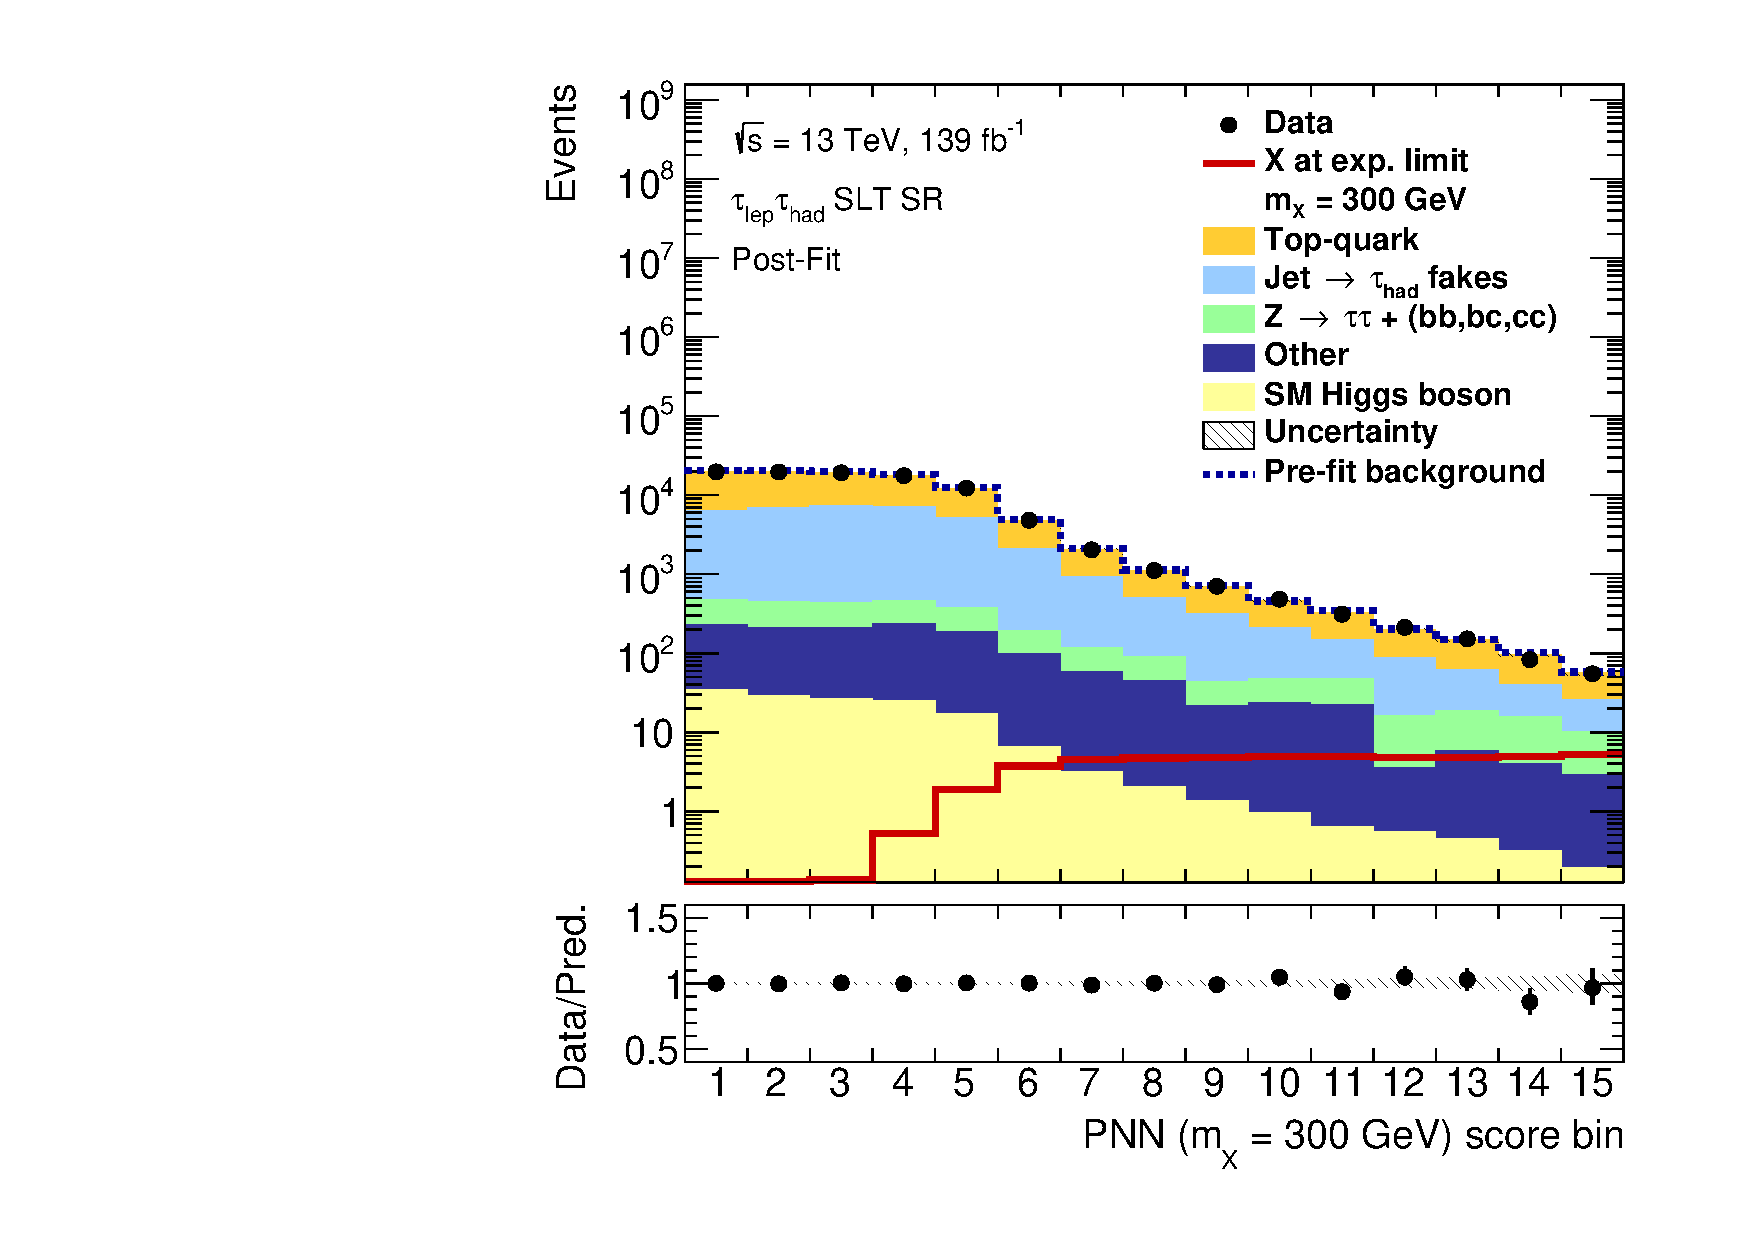
\includegraphics[width=\textwidth]{results_res/postfit/Region_BMin0_incJet1_dist300_J2_D2HDMPNN_T2_SpcTauLH_Y2015_LTT0_L1_GlobalFit_conditionnal_mu0log}
    \subcaption{$\mX = \SI{300}{\GeV}$}
  \end{subfigure}\hfill%
  \begin{subfigure}{0.495\textwidth}
    \centering

    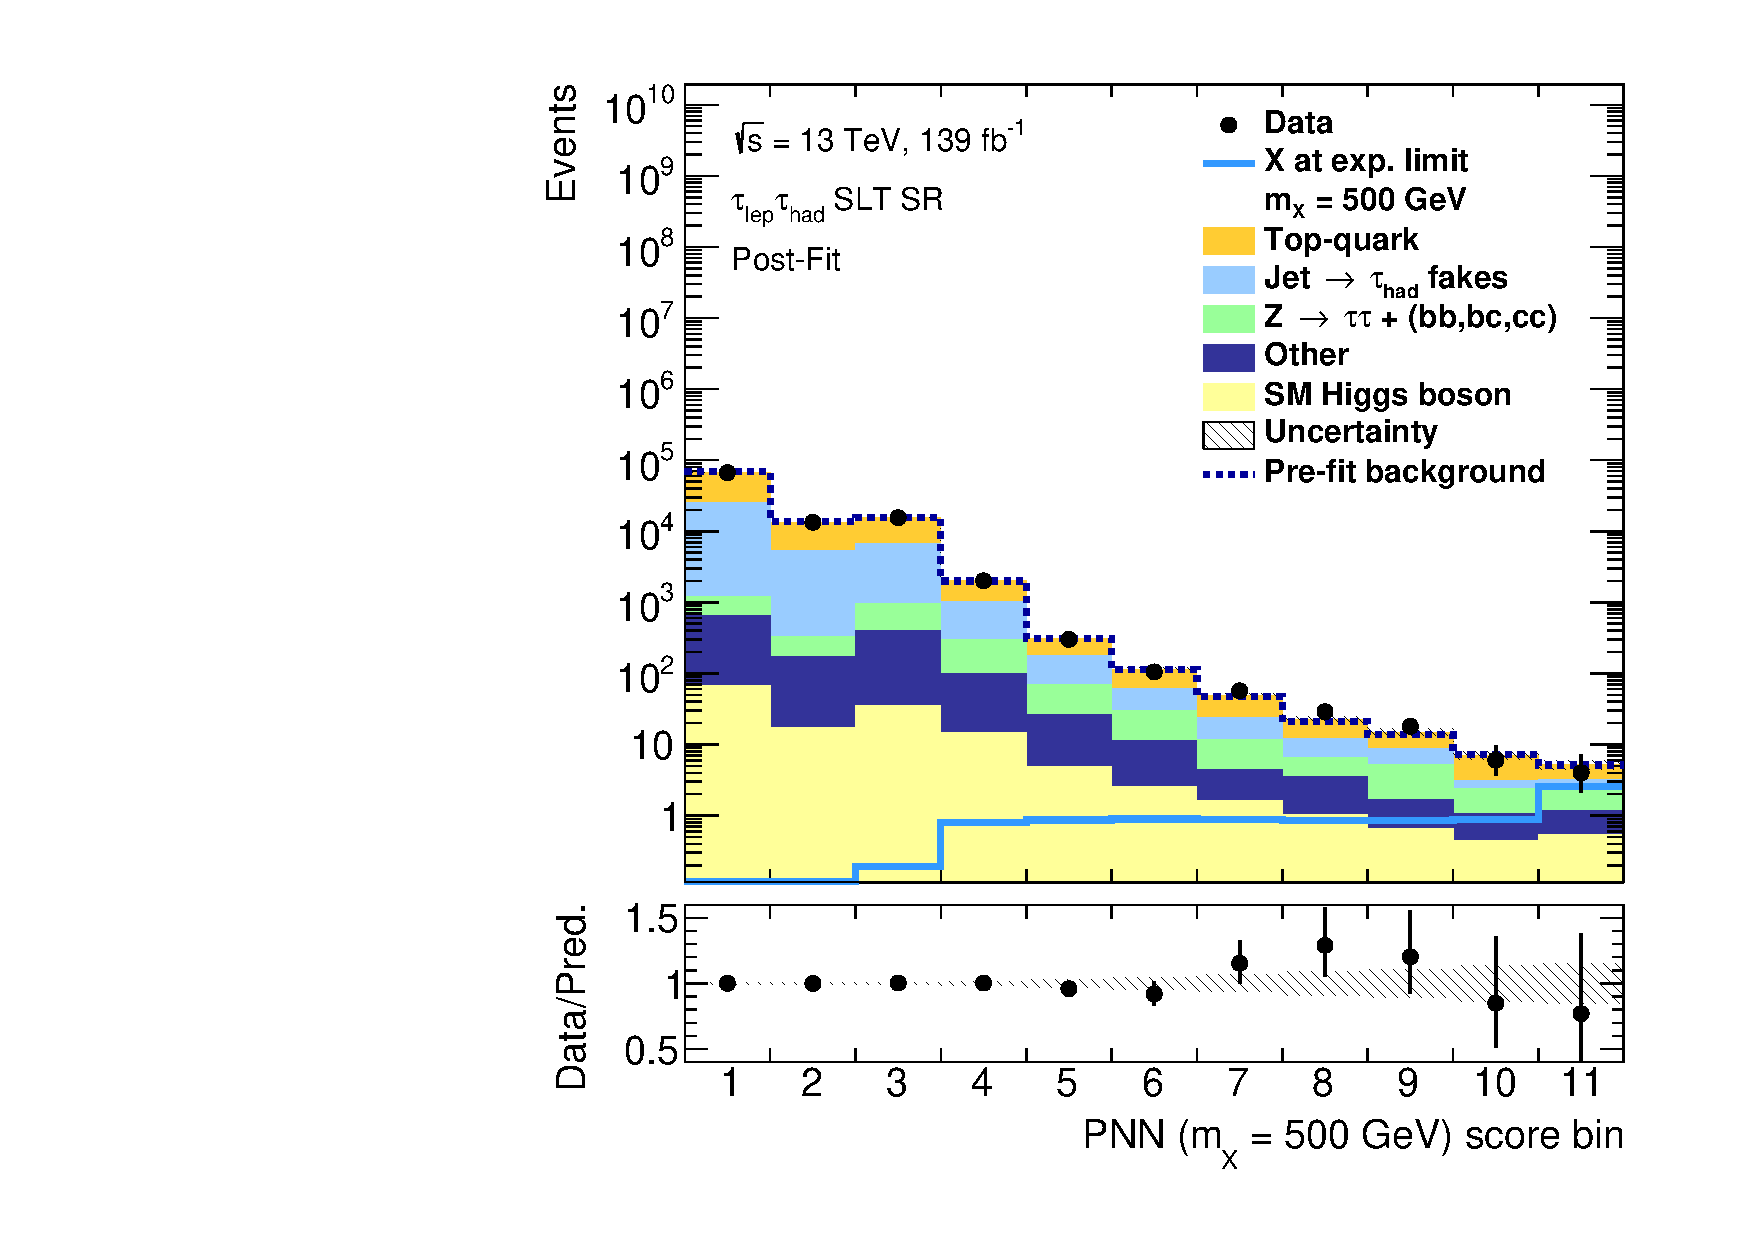
\includegraphics[width=\textwidth]{results_res/postfit/Region_BMin0_incJet1_dist500_J2_D2HDMPNN_T2_SpcTauLH_Y2015_LTT0_L1_GlobalFit_conditionnal_mu0log}
    \subcaption{$\mX = \SI{500}{\GeV}$}
  \end{subfigure}

  \begin{subfigure}{0.495\textwidth}
    \centering

    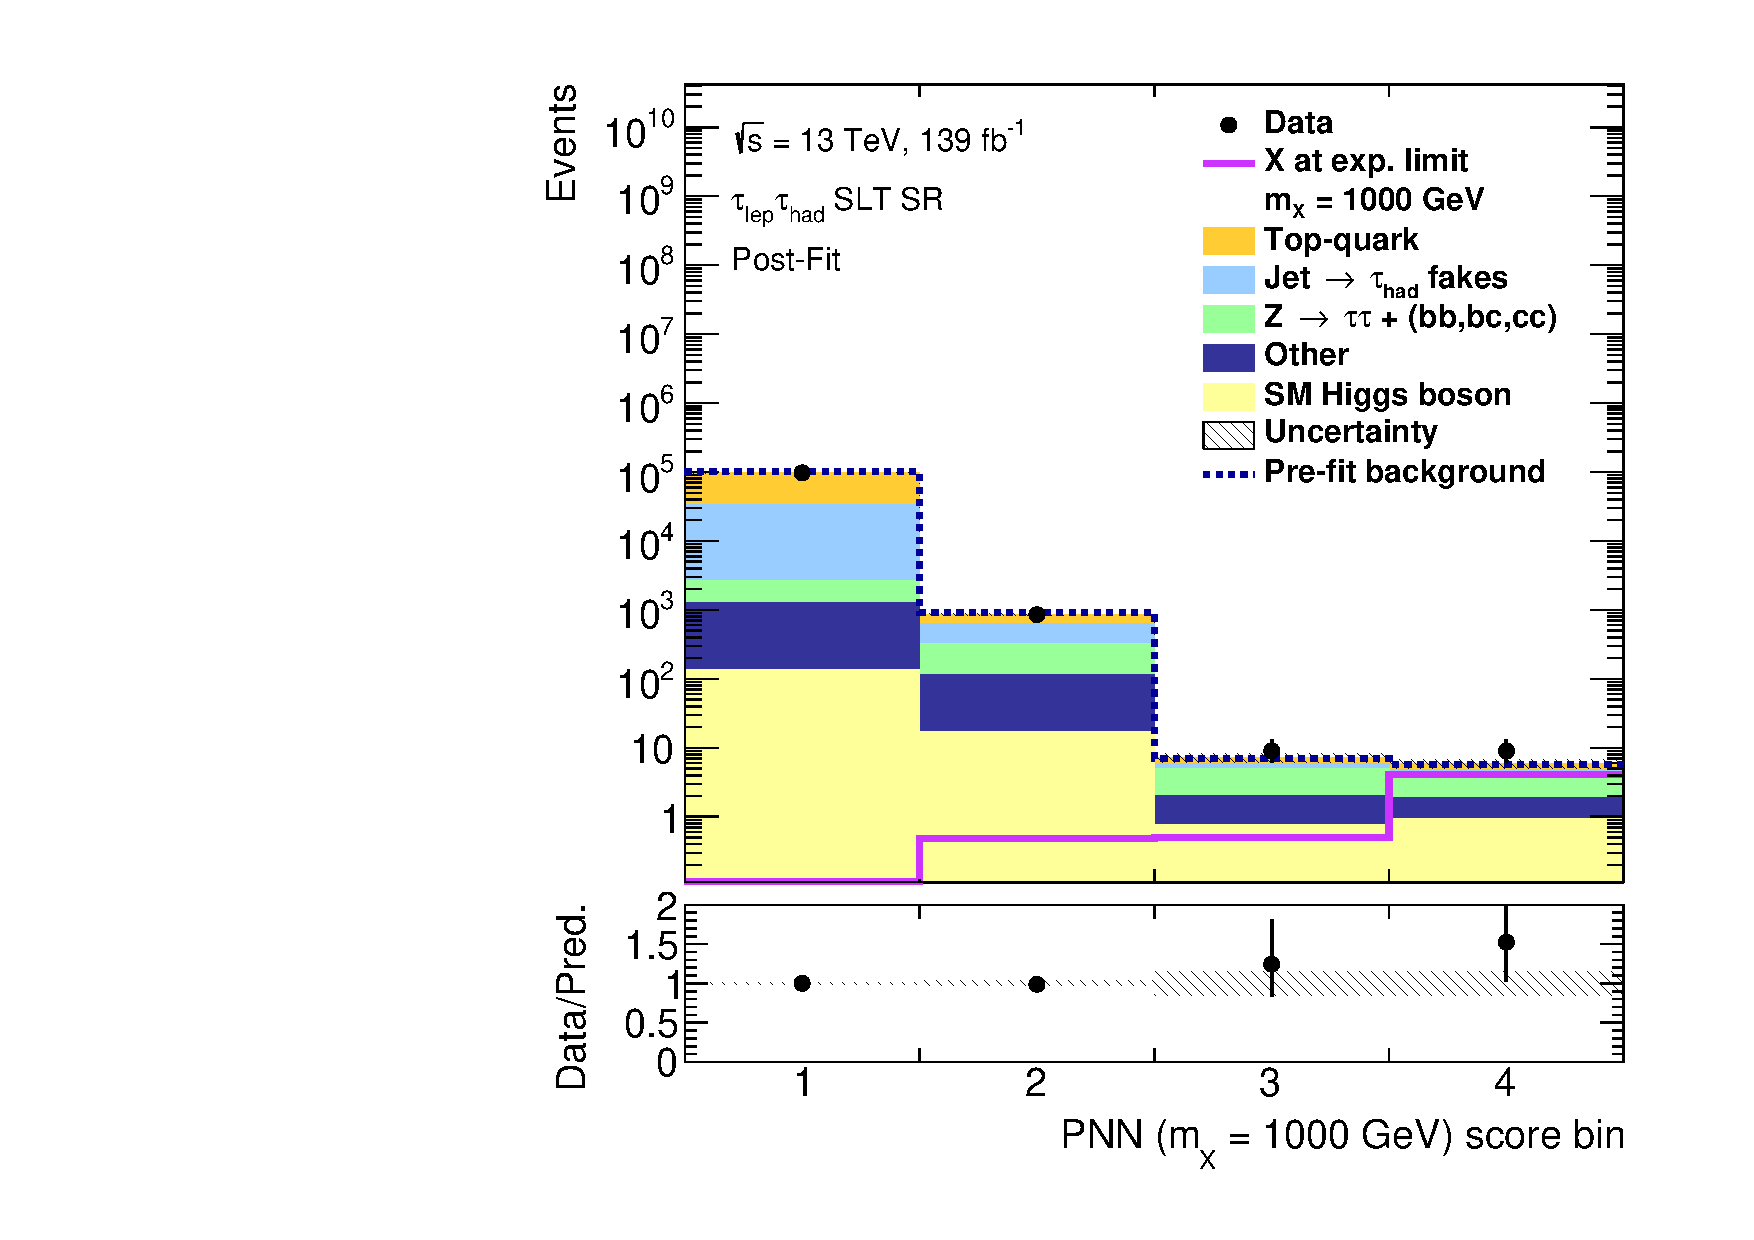
\includegraphics[width=\textwidth]{results_res/postfit/Region_BMin0_incJet1_dist1000_J2_D2HDMPNN_T2_SpcTauLH_Y2015_LTT0_L1_GlobalFit_conditionnal_mu0log}
    \subcaption{$\mX = \SI{1000}{\GeV}$}
  \end{subfigure}\hfill%
  \begin{subfigure}{0.495\textwidth}
    \centering

    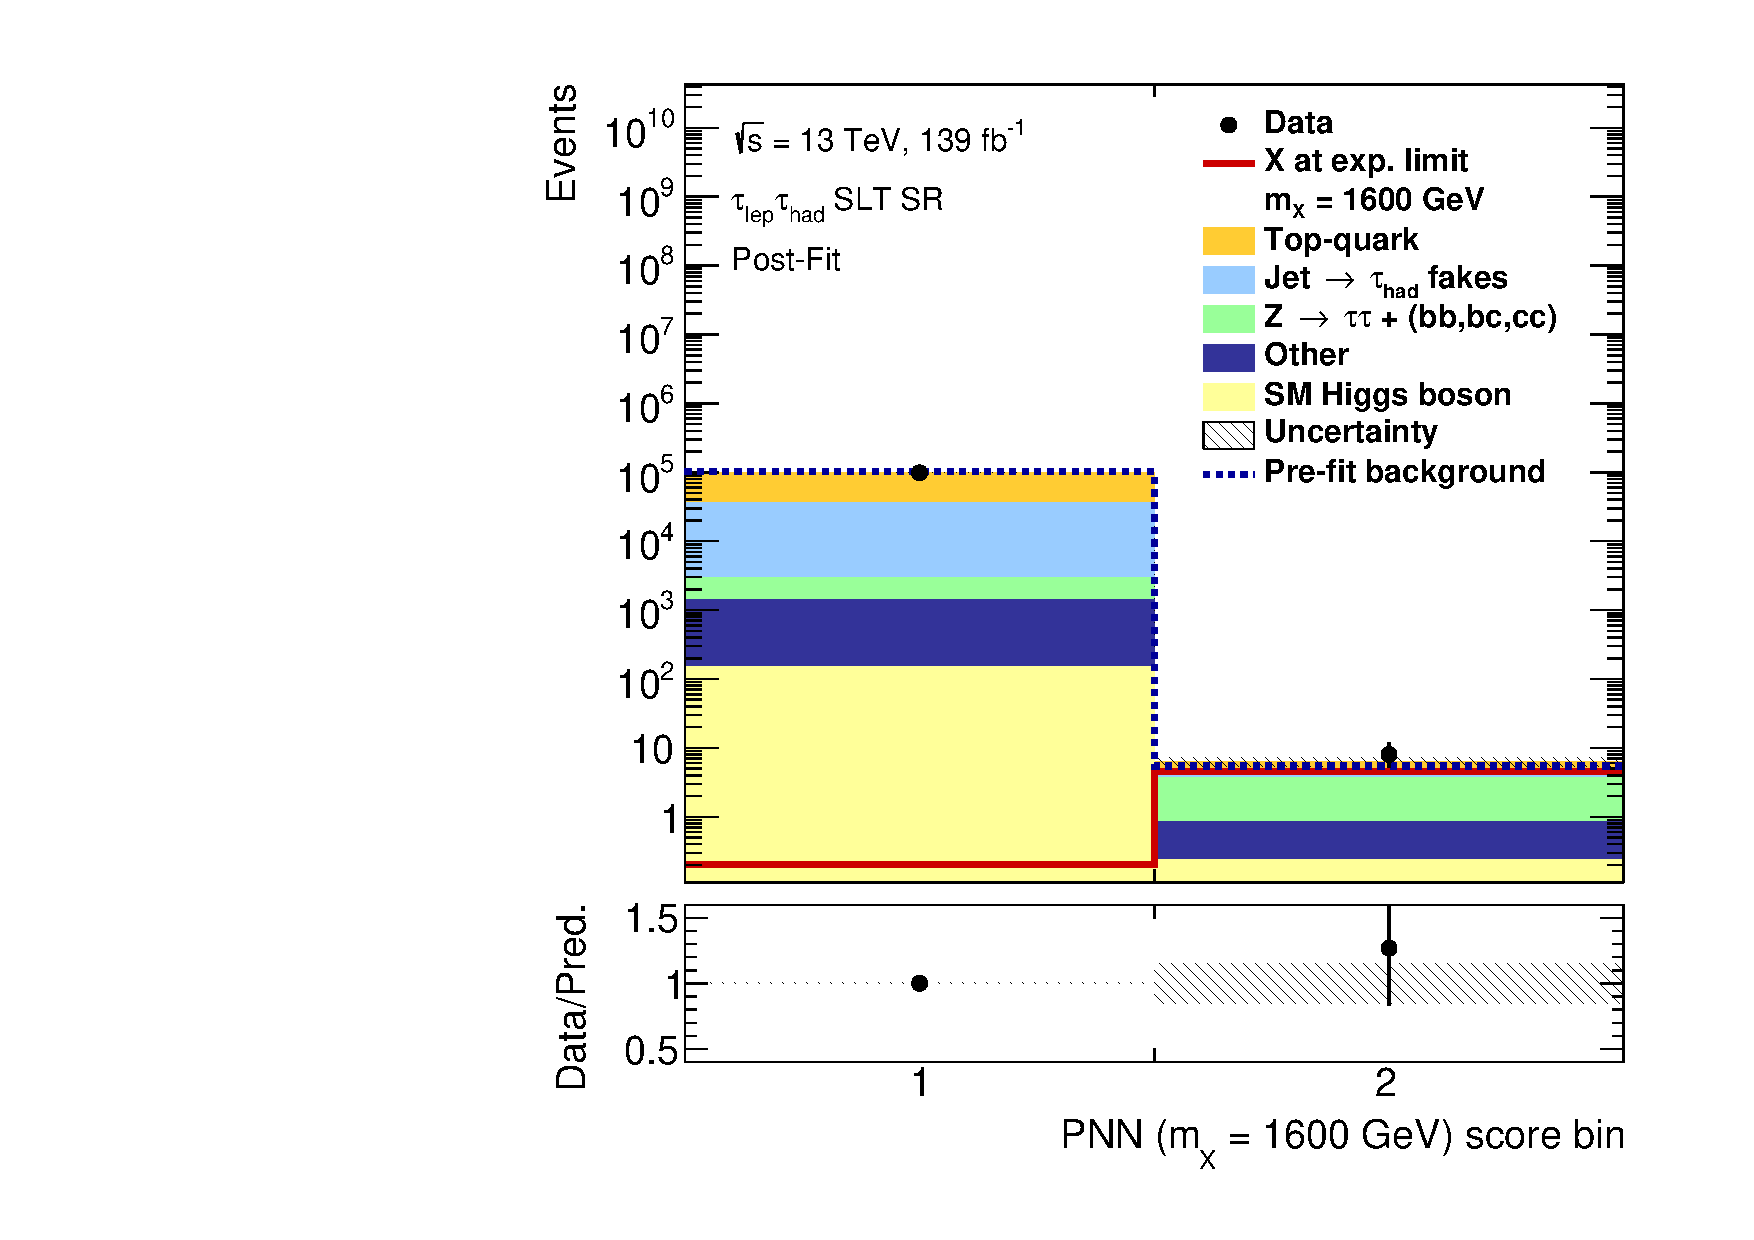
\includegraphics[width=\textwidth]{results_res/postfit/Region_BMin0_incJet1_dist1600_J2_D2HDMPNN_T2_SpcTauLH_Y2015_LTT0_L1_GlobalFit_conditionnal_mu0log}
    \subcaption{$\mX = \SI{1600}{\GeV}$}
  \end{subfigure}

  \caption{Distribution of the PNN discriminant of the \lephad SLT channel after
    the maximum likelihood fit of the background-only model in all SRs and
    CRs. The signal overlay is scaled to the expected upper limit on
    $\sigma(pp \to X \to HH)$.}
\end{figure}


\begin{figure}[htbp]
  \centering

  \begin{subfigure}{0.495\textwidth}
    \centering

    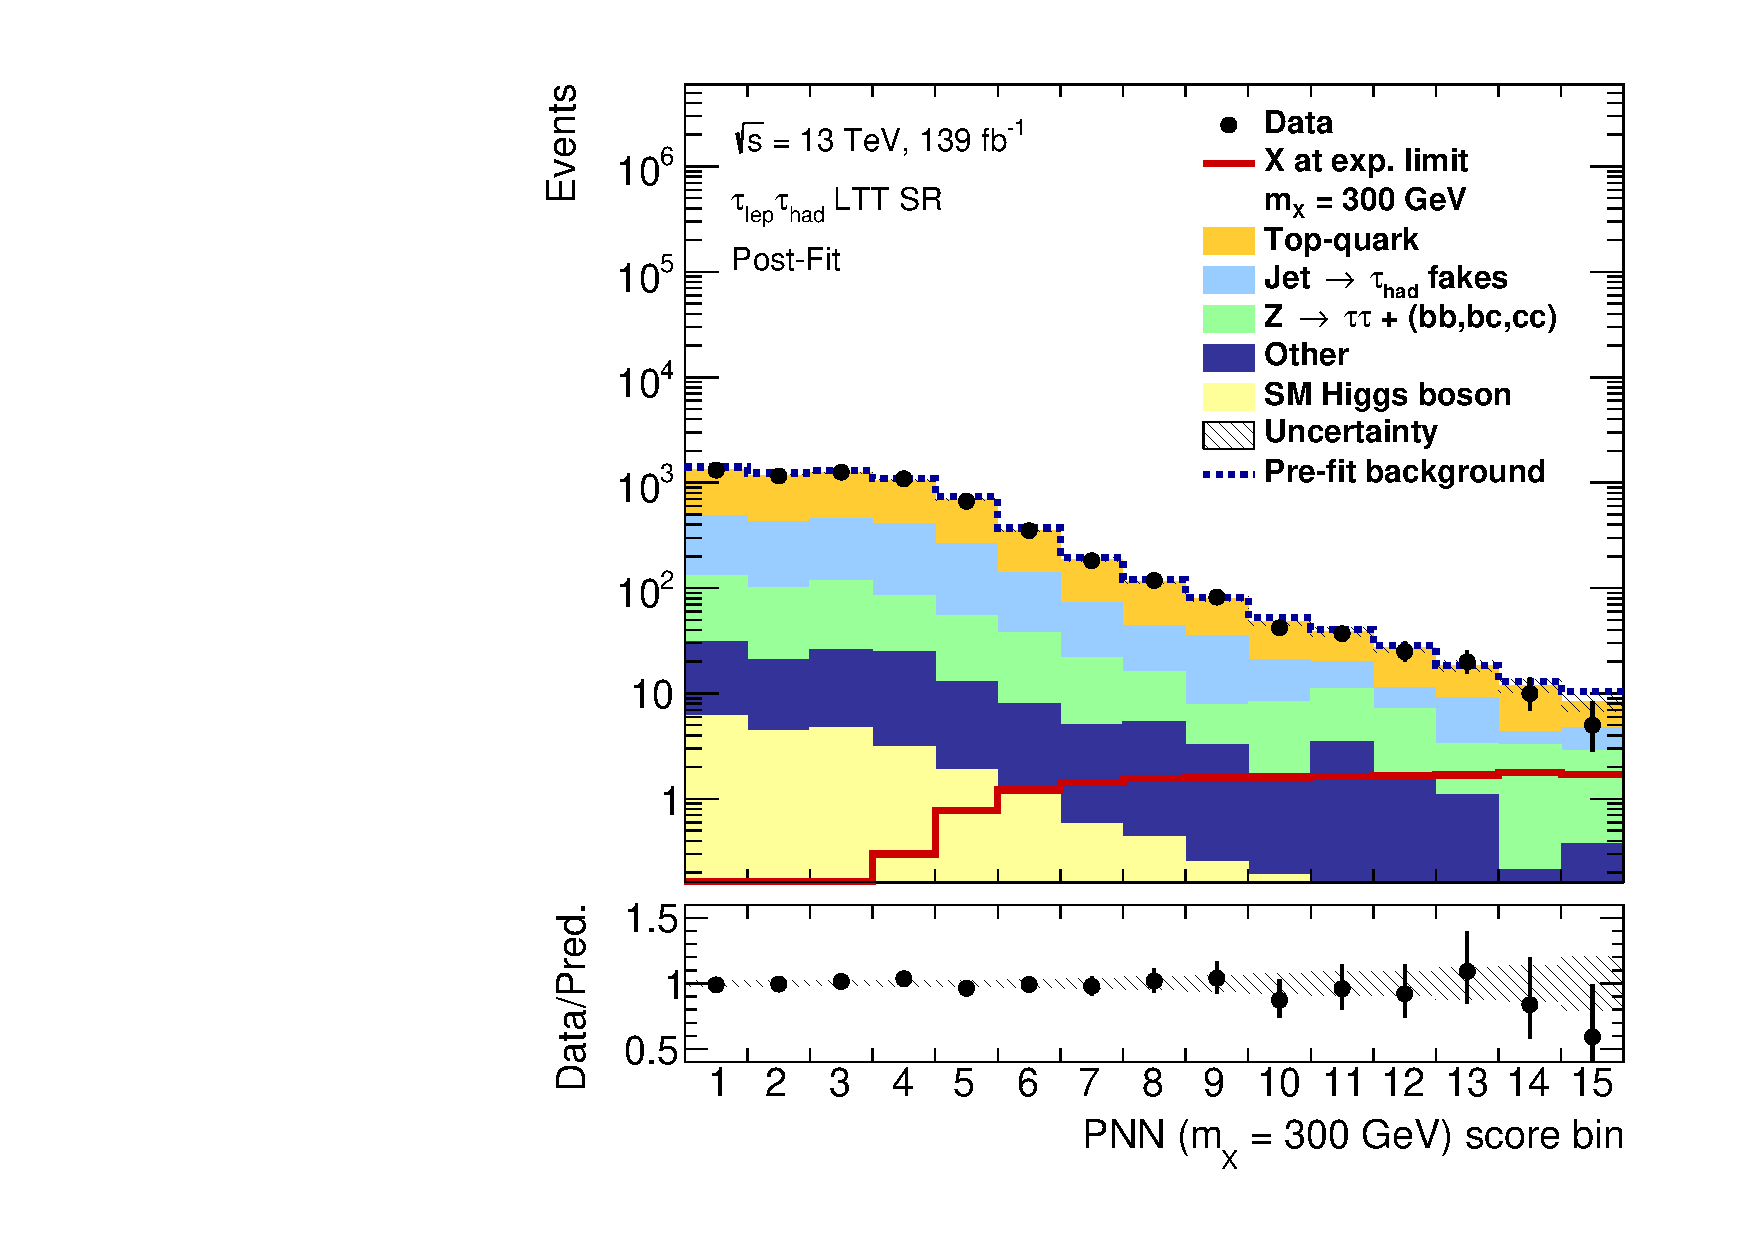
\includegraphics[width=\textwidth]{results_res/postfit/Region_BMin0_incJet1_dist300_J2_D2HDMPNN_T2_SpcTauLH_Y2015_LTT1_L1_GlobalFit_conditionnal_mu0log}
    \subcaption{$\mX = \SI{300}{\GeV}$}
  \end{subfigure}\hfill%
  \begin{subfigure}{0.495\textwidth}
    \centering

    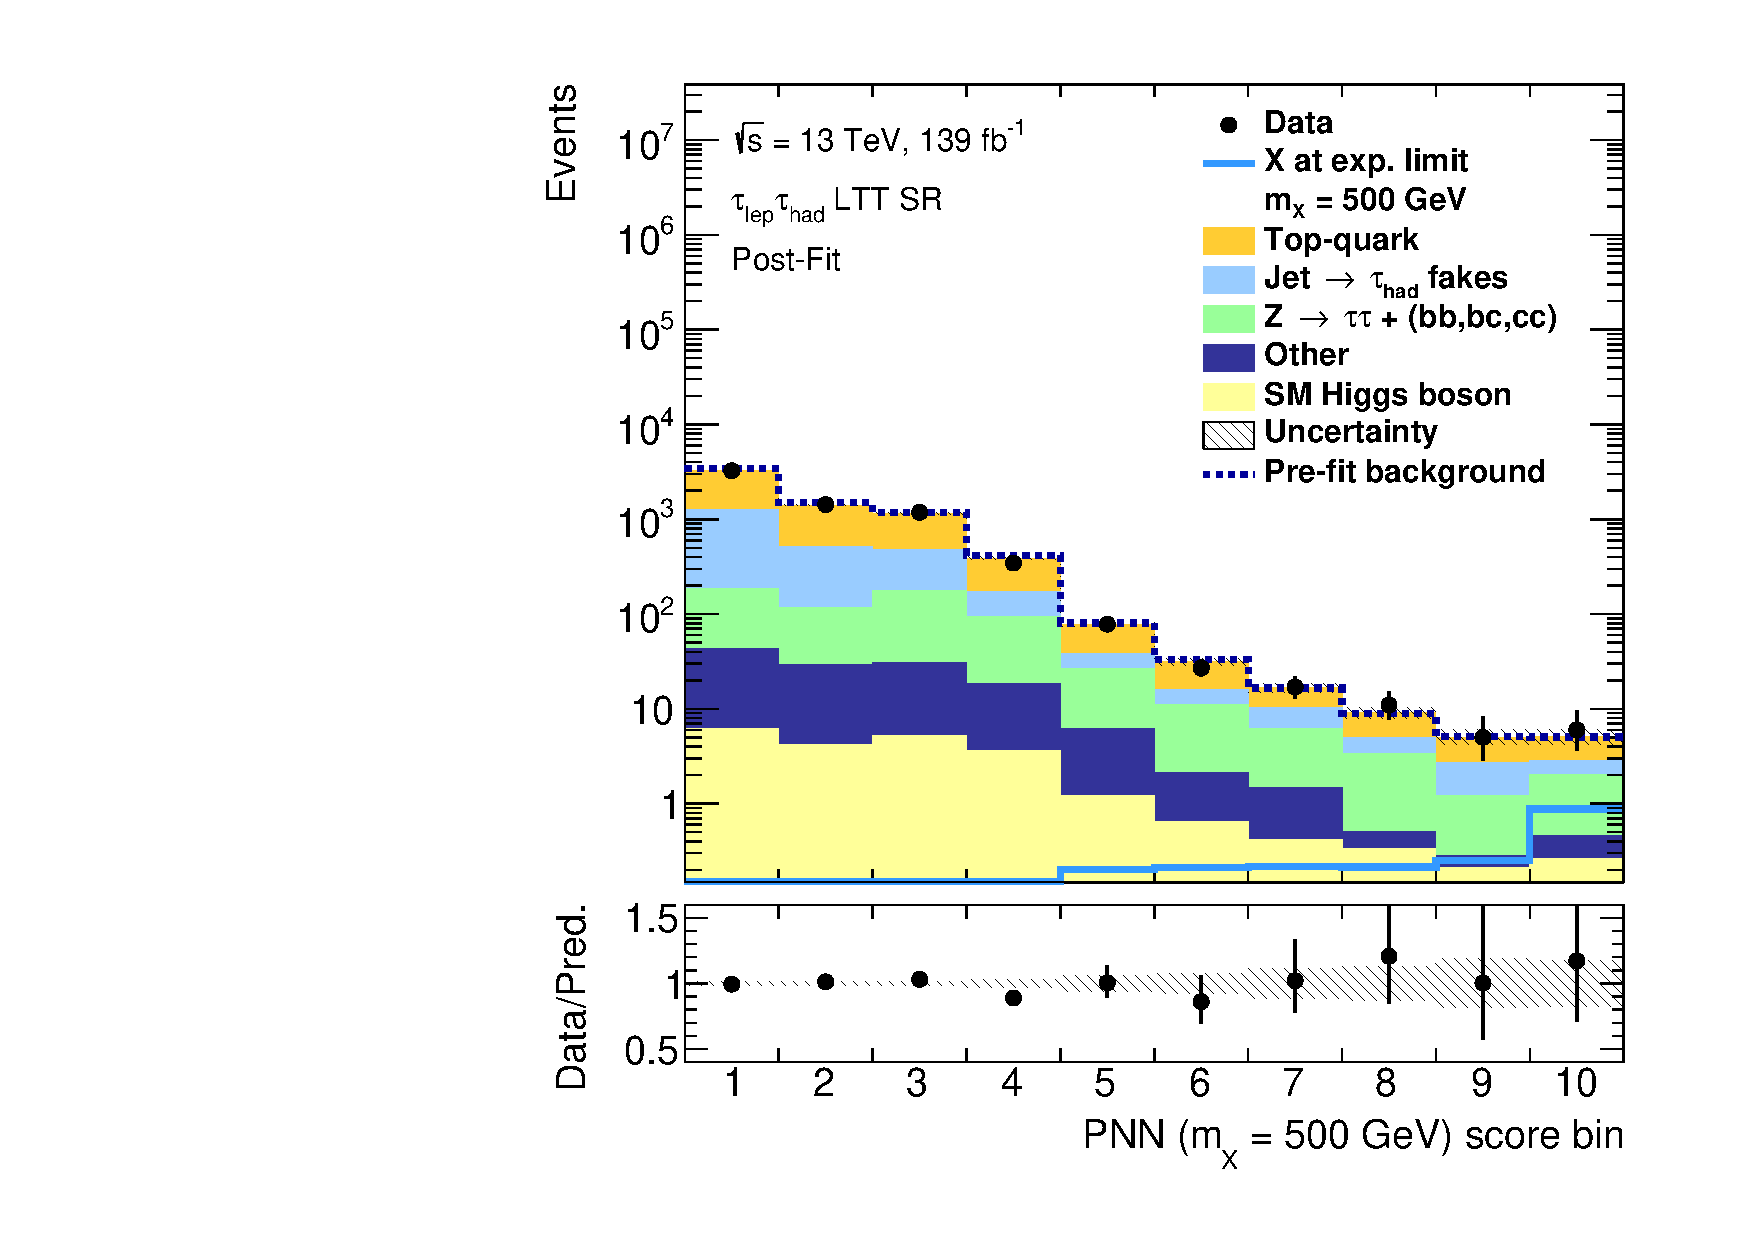
\includegraphics[width=\textwidth]{results_res/postfit/Region_BMin0_incJet1_dist500_J2_D2HDMPNN_T2_SpcTauLH_Y2015_LTT1_L1_GlobalFit_conditionnal_mu0log}
    \subcaption{$\mX = \SI{500}{\GeV}$}
  \end{subfigure}

  \begin{subfigure}{0.495\textwidth}
    \centering

    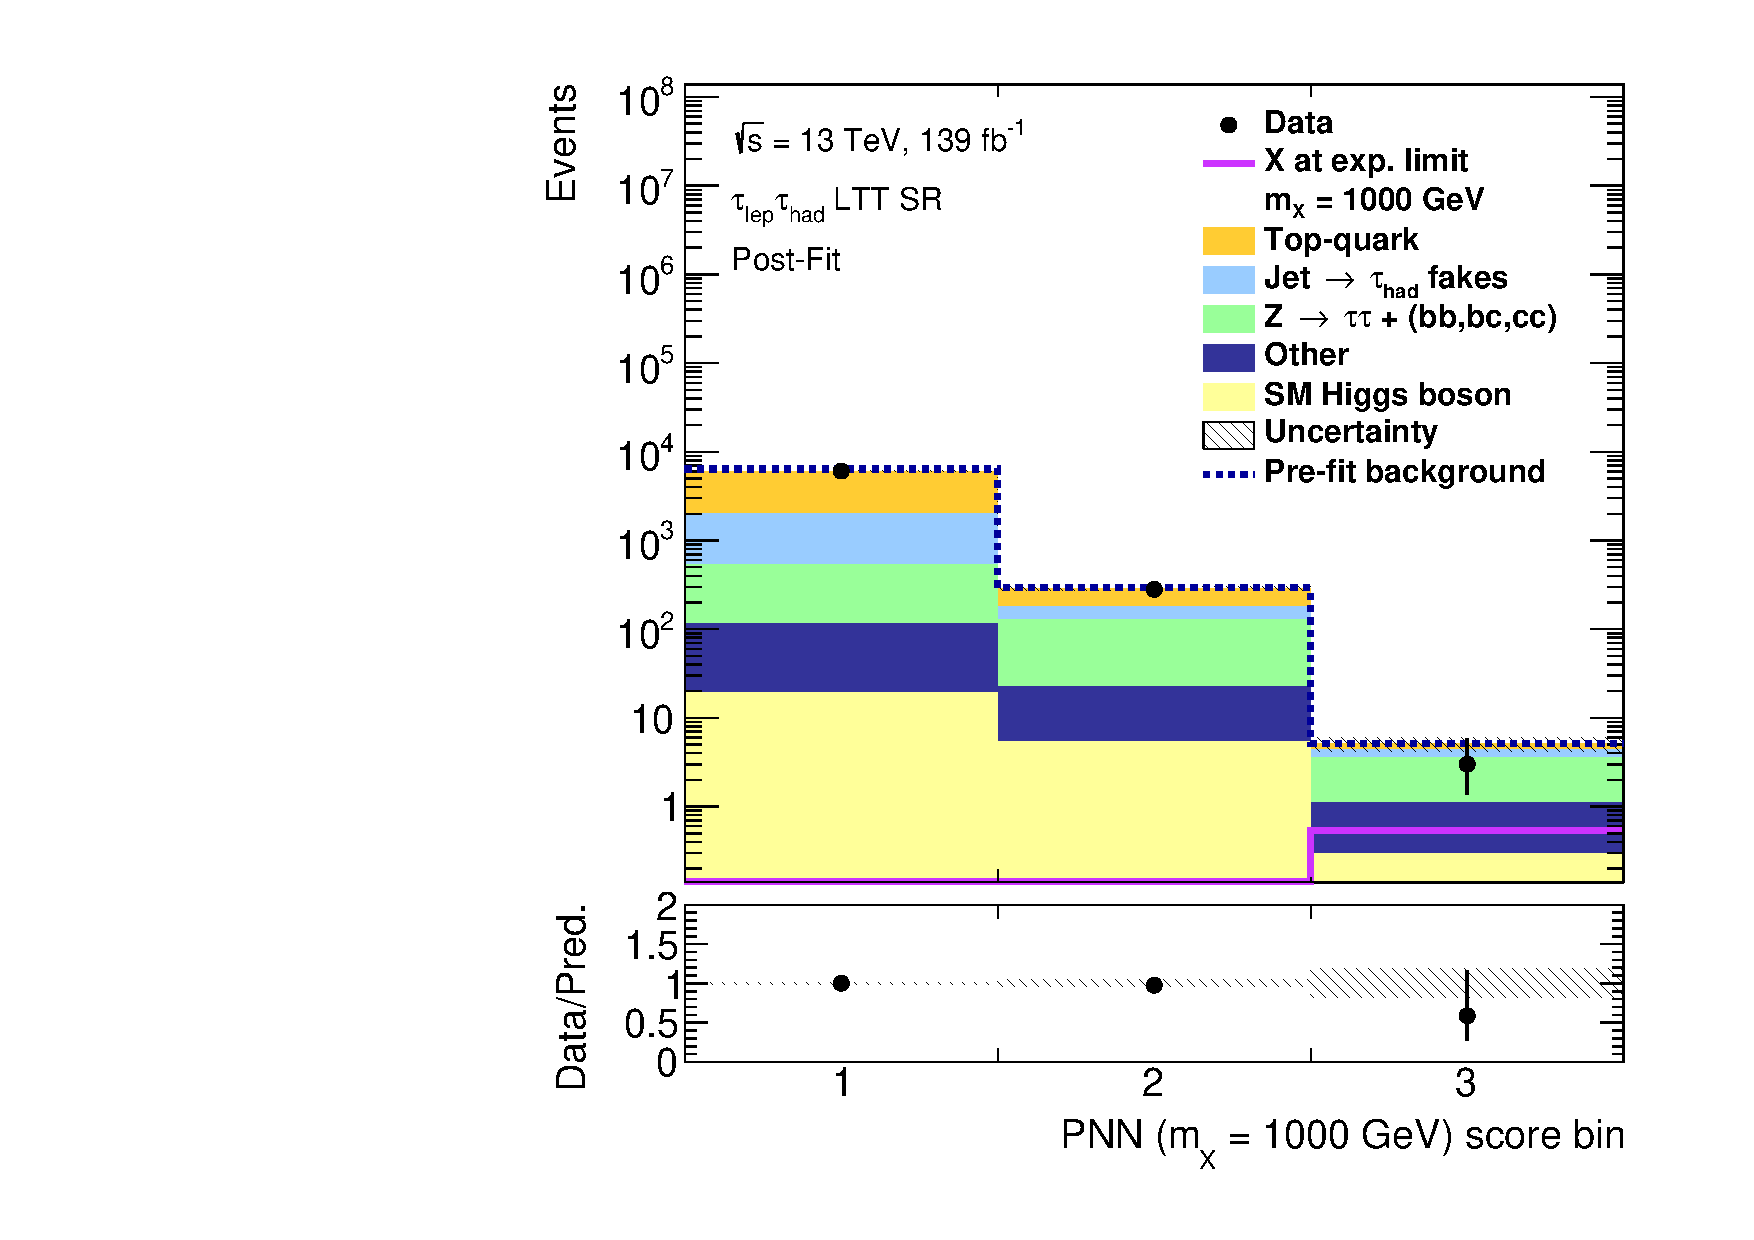
\includegraphics[width=\textwidth]{results_res/postfit/Region_BMin0_incJet1_dist1000_J2_D2HDMPNN_T2_SpcTauLH_Y2015_LTT1_L1_GlobalFit_conditionnal_mu0log}
    \subcaption{$\mX = \SI{1000}{\GeV}$}
  \end{subfigure}\hfill%
  \begin{subfigure}{0.495\textwidth}
    \centering

    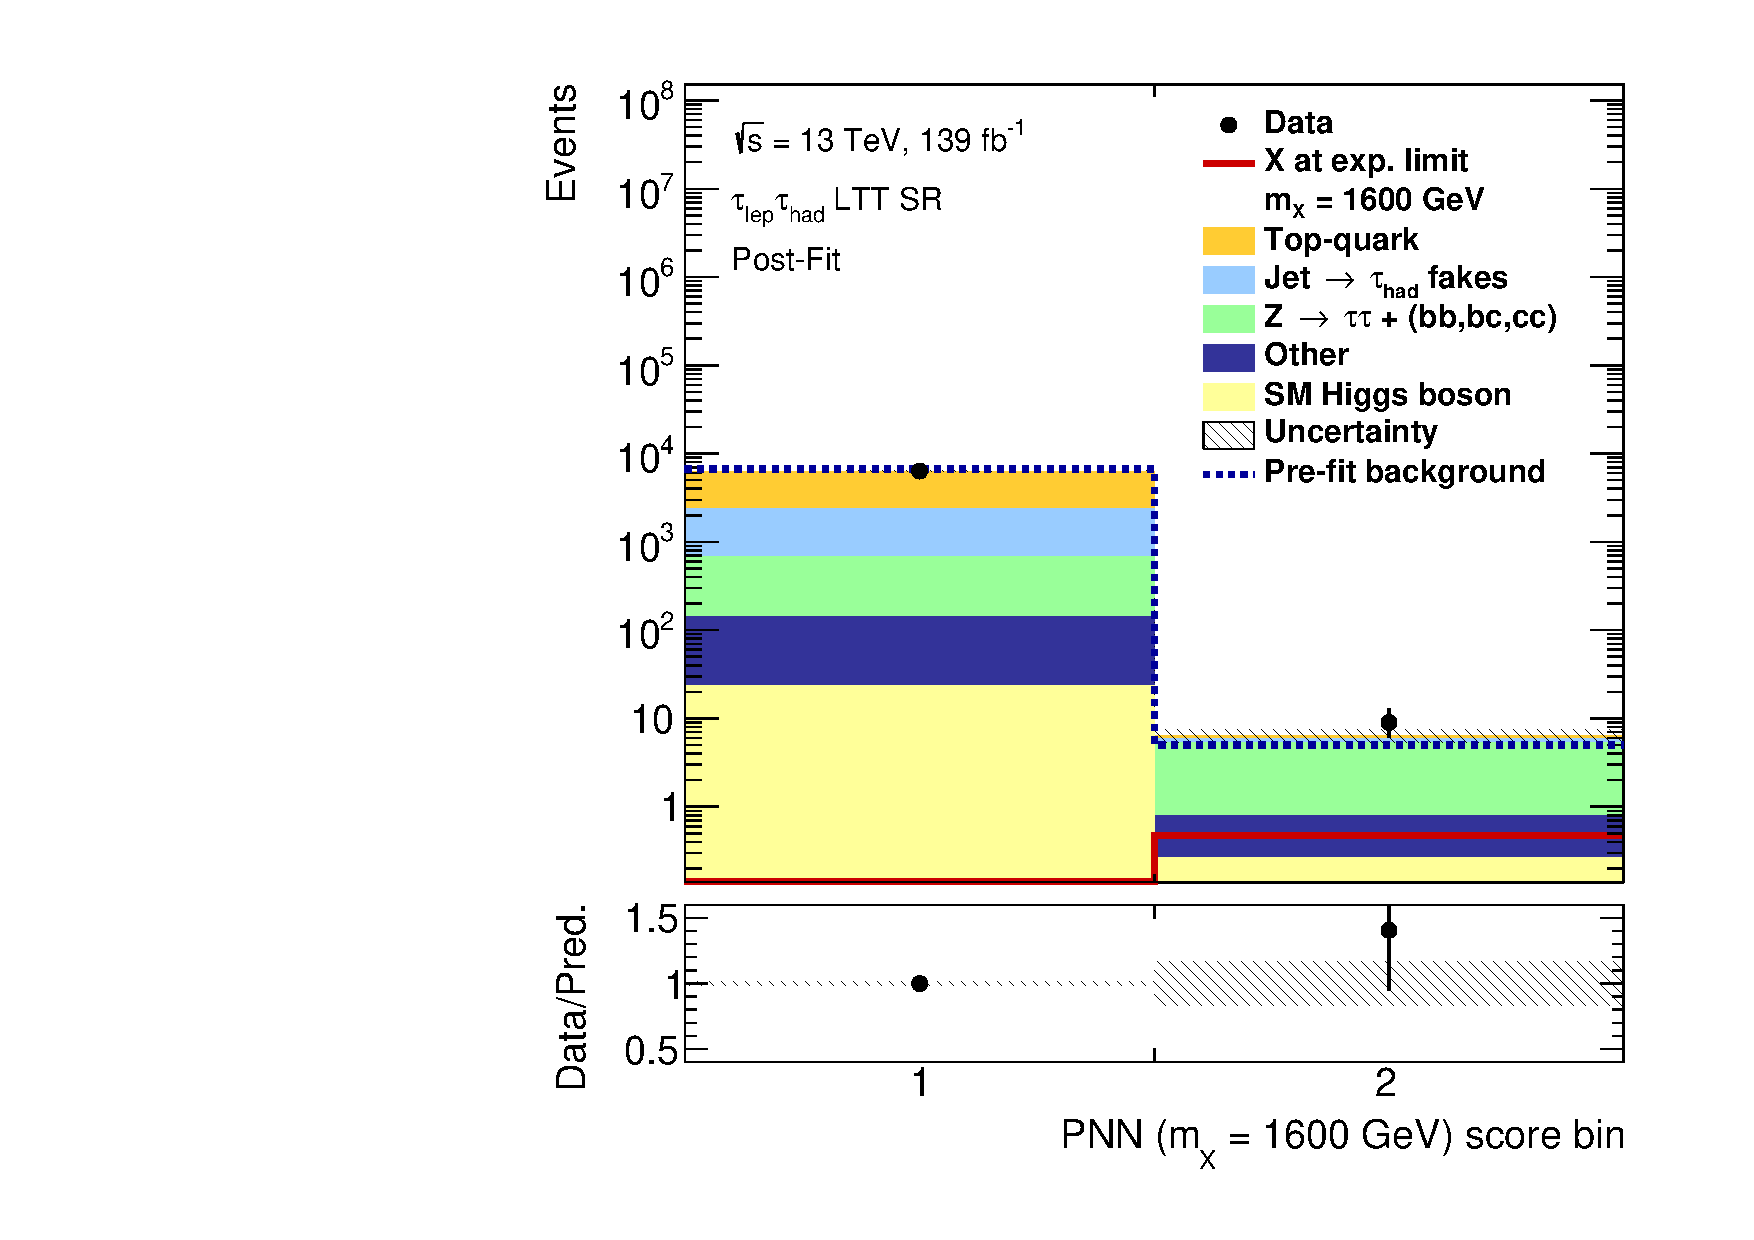
\includegraphics[width=\textwidth]{results_res/postfit/Region_BMin0_incJet1_dist1600_J2_D2HDMPNN_T2_SpcTauLH_Y2015_LTT1_L1_GlobalFit_conditionnal_mu0log}
    \subcaption{$\mX = \SI{1600}{\GeV}$}
  \end{subfigure}

  \caption{Distribution of the PNN discriminant of the \lephad LTT
    channel after the maximum likelihood fit of the background-only
    model in all SRs and CRs. The signal overlay is
    scaled to the expected upper limit on $\sigma(pp \to X \to HH)$.}
\end{figure}


% ------------------------------------------------------------------------------
\clearpage
\subsection{Breakdown}%
\label{app:breakdown_table}
% ------------------------------------------------------------------------------

\begin{table}[htbp]
  \centering

  \caption{Decomposition of the variance on $\hat{\sigma}$, the
    maximum likelihood estimate of the cross section
    $\sigma(pp \to X\to HH)$, by uncertainty category for the fit to
    Asimov data with $\mu = 0$ in all regions. The decomposition is
    determined analogously to~\Cref{tab:breakdown_nonres}, separately
    for four exemplary signal mass hypotheses. The fractions of
    subcategories do not necessarily sum to the fraction of the parent
    category due to correlations between nuisance parameters.}%
  \label{tab:breakdown_res_exp_mu0}

  \begin{tabular}{
  l
  S[table-format=2.0, table-space-text-pre=\textless, table-column-width=1.6cm]
  S[table-format=2.0, table-space-text-pre=\textless, table-column-width=1.6cm]
  S[table-format=2.0, table-space-text-pre=\textless, table-column-width=1.6cm]
  S[table-format=2.0, table-space-text-pre=\textless, table-column-width=1.6cm]
  }
  \toprule
         & \multicolumn{4}{c}{Explained fraction of variance on $\hat{\sigma}$}\\
         %& \multicolumn{4}{c}{of variance on $\hat{\mu}$}\\
  \cmidrule{2-5}
  Source & {$\SI{300}{\GeV}$} & {$\SI{500}{\GeV}$} & {$\SI{1000}{\GeV}$} & {$\SI{1600}{\GeV}$} \\
  \midrule
  \textbf{Data statistical uncertainty}
         & 59\,\si{\percent} & 81\,\si{\percent} & 82\,\si{\percent} & 82\,\si{\percent} \\
  \textbf{Systematic uncertainties}
         & 41\,\si{\percent} & 19\,\si{\percent} & 18\,\si{\percent} & 17\,\si{\percent} \\
  \hspace{0.8em} Instrumental uncertainties
         & 10\,\si{\percent} & 1\,\si{\percent} & 1\,\si{\percent} & {\textless} 1\,\si{\percent}\\
  \hspace{0.8em} Signal modelling uncertainties
         & 1\,\si{\percent}  & 1\,\si{\percent} & {\textless} 1\,\si{\percent} & 3\,\si{\percent} \\
  \hspace{0.8em} Background statistical uncertainties
         & 18\,\si{\percent} & 11\,\si{\percent} & 7\,\si{\percent} & 9\,\si{\percent} \\
  \hspace{0.8em} Background modelling uncertainties
         & 12\,\si{\percent} & 7\,\si{\percent} & 10\,\si{\percent} & 5\,\si{\percent} \\
  \midrule
  \hspace{1.6em} -- \hspace{0.2em} Top-quark (incl.\ free normalisation)
         & 3\,\si{\percent} & 2\,\si{\percent} & 1\,\si{\percent} & {\textless} 1\,\si{\percent} \\
  \hspace{1.6em} -- \hspace{0.2em} \ZHF (incl.\ free normalisation)
         & 3\,\si{\percent} & 1\,\si{\percent} & 3\,\si{\percent} & 2\,\si{\percent} \\
  \hspace{1.6em} -- \hspace{0.2em} SM Higgs boson
         & {\textless} 1\,\si{\percent} & 2\,\si{\percent} & 3\,\si{\percent} & 2\,\si{\percent} \\
  \hspace{1.6em} -- \hspace{0.2em} Fake-\tauhadvis
         & 4\,\si{\percent} & {\textless} 1\,\si{\percent} & 1\,\si{\percent} & 1\,\si{\percent} \\
  \hspace{1.6em} -- \hspace{0.2em} Other
         & {\textless} 1\,\si{\percent} & {\textless} 1\,\si{\percent} & {\textless} 1\,\si{\percent} & {\textless} 1\,\si{\percent} \\
  \bottomrule
\end{tabular}

%%% Local Variables:
%%% mode: latex
%%% TeX-master: "../phd_thesis"
%%% End:

\end{table}


%%% Local Variables:
%%% mode: latex
%%% TeX-master: "../../phd_thesis"
%%% End:
